\chapter{Results}\label{chap3}
\thispagestyle{plain}

In this section I will report the statistics of the RADNET dataset leading to the choice of the weights for the cross-entropy loss. The distribution of rainfall rates is assessed. Finally, I give the final results for the relevant classification task.
% ==== SECTION 1 ===============================================================
\section{Dataset Statistics}
Rainfall patterns vary greatly from location to location which in turn affects the distribution and frequency of the precipitation rainfall rates picked up through radar. The RADOLAN dataset is no exception. Given that this project has as goal to replicate to some extent the model by \citet{Agrawal2019MachineImages} I verify that induced choices are at least to a first glance acceptable. When it comes to dividing rainfall into classes for the classification problem \citet{Agrawal2019MachineImages} decides to adopt three different thresholds for this subdivision. These are 0.1 mm/h, 1 mm/h and 2.5 mm/h. However, differences in the structure of the problem of this project and the one by \citet{Agrawal2019MachineImages} exist. (1) The categorization problem by \citet{Agrawal2019MachineImages} outputs images that are compared with radar derived precipitation estimates at 1 h. These estimates are outputted every 10min. Conversely, for this project both the inputs and outputs are given every at an hourly rate from each other. (2) \citet{Agrawal2019MachineImages} structures the problem as multiple binary classification tasks whereas this project is structured as one single multi-class classification task. (3) Oversampling frames with precipitation is the method used by \citet{Agrawal2019MachineImages} to compensate for the fact that the majority of pixels is rainless. In this project I simply ignore the scenes where all of the input frames have no rainy pixel. I also add weights to the simple cross-entropy loss.

The analysis of the dataset then yields class distributions for the different dataset subsets (training, validation, testing) as in \cref{tab:classdistributions} and in \cref{fig:classdistributions}. A summary of the percentages of scenes used out of all scenes available and their final proportion in the dataset is given in \cref{tab:rainydays}.
\begin{table}[h]
    \centering
    \begin{tabular}{ccccc}
    \hline
         \multicolumn{5}{c}{Frequency \% Classes}  \\
         \hline
         \hline
         Class Label & Class Interval & Training & Validation & Test \\
         \hline
         0 & $[0, 0.1)$ & 89.4\% & 88.02\% & 87.78\% \\
         0.1 & $[0.1, 1.0)$ & 8.34\% & 9.46\% & 9.57\% \\
         1.0 & $[1.0, 2.5)$ & 1.81\% & 2.05\% & 2.2\%  \\
         2.5 & $[2.5, \infty)$ & 0.42\% & 0.47\% & 0.45\% \\
         \hline
    \end{tabular}
    \caption{Frequencies of the different classes in the target channel for every subset of the dataset. The class frequencies for the training subset are used to determine the weights for the weighted cross-entropy loss. A bar chart from the data contained in this table is depicted in \cref{fig:classdistributions}.}
    \label{tab:classdistributions}
\end{table}
\begin{figure}[h]
    \centering
    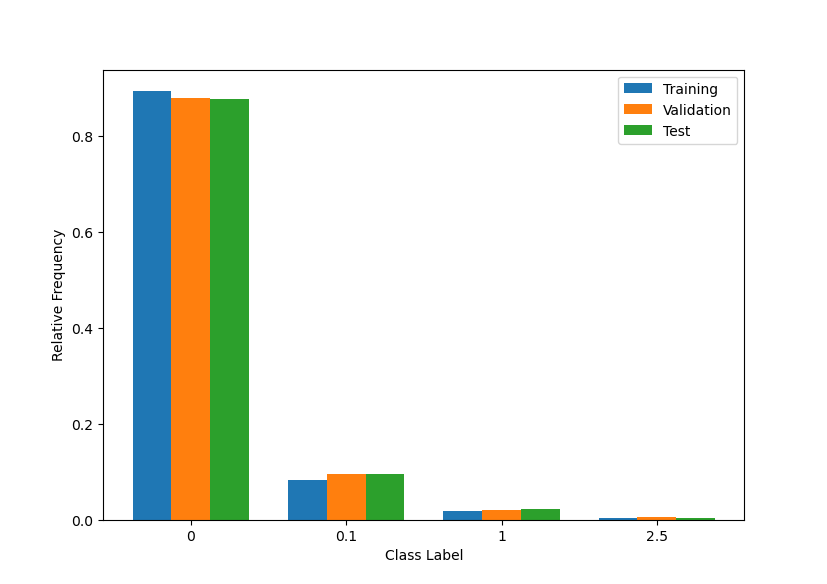
\includegraphics[width=0.9\textwidth]{Class Frequencies Bar.png}
    \caption{Bar chart of the precipitation class (see \cref{tab:prec_classes}) frequencies for training, validation and test subset of the dataset. The frequencies sum to 1 for each one of the subsets. The chart is computed using data from \cref{tab:classdistributions}.}
    \label{fig:classdistributions}
\end{figure}
\begin{table}[h]
    \centering
    \begin{tabular}{cccc}
    \hline
    \multicolumn{4}{c}{Scenes Selection} \\
    \hline
    \hline
         & Training & Validation & Test \\
    \hline
         Available Scenes & 63336 & 10176 & 10200 \\
         Selected Scenes & 58784 & 7116 & 7074 \\
         Percentage Selected & 92.8\% & 69.9\% & 69.3\% \\
         Proportion in Dataset & 80.6\% & 9.8\% & 9.7\% \\
         \hline
    \end{tabular}
    \caption{Breakdown of the selection of scenes from all the available scenes. The third row is computed by dividing the selected scenes by the available scenes. The proportion in the total dataset is computed by dividing the selected scenes by the sum of all selected scenes. A scene is discarded if and only if all the input frames are rainless.}
    \label{tab:rainydays}
\end{table}


\subsubsection{Weights for Training}
To counteract the class imbalance, using weights in the cross-entropy loss of the model is normally the preferred choice in the deep learning literature. These weights are typically the inverse of the frequency of the classes. That means, following the frequencies as reported in \cref{tab:classdistributions},
\begin{align*}
   & \text{Class 0} & \frac{1}{89.4} \\
   & \text{Class 0.1} & \frac{1}{8.34} \\
   & \text{Class 1.0} & \frac{1}{1.81} \\
   & \text{Class 2.5} & \frac{1}{0.42}
\end{align*}
Other methods of balancing a cross-entropy loss exist, such as the employment of an effective number of samples \citep{Cui2019Class-BalancedSamples} that builds upon the reasoning that as the number of samples increases, the additional benefit of a newly added data point diminishes.
\subsubsection{Skewness of inputs}
Knowing that high precipitation rates are infrequent and that in general very skewed distributions for the layers of a neural network are not desireable, I assess the frequency and shape of the distribution of the values for the raw precipitation rates of the RADOLAN dataset as those are the ones that are fed as input to the model. 

In order to make the distribution less skewed and bring it closer to a normal distribution, a common solution is to transform the data by taking the (natural) logarithm; for instance \citet{Ayzel2020RainNetNowcasting} decide to transform the input to the model by taking the natural logarithm as in
\begin{equation} \label{eq:transform}
    x_{\text{transformed}} = \ln(x_{raw} + 0.01)
\end{equation}
where 0.01 is added to the raw input to avoid the logarithm of zero. \cref{fig:trainfreq} shows the implication of this transformation for the distribution of the precipitation values.

\begin{figure}[!h]
    \centering
    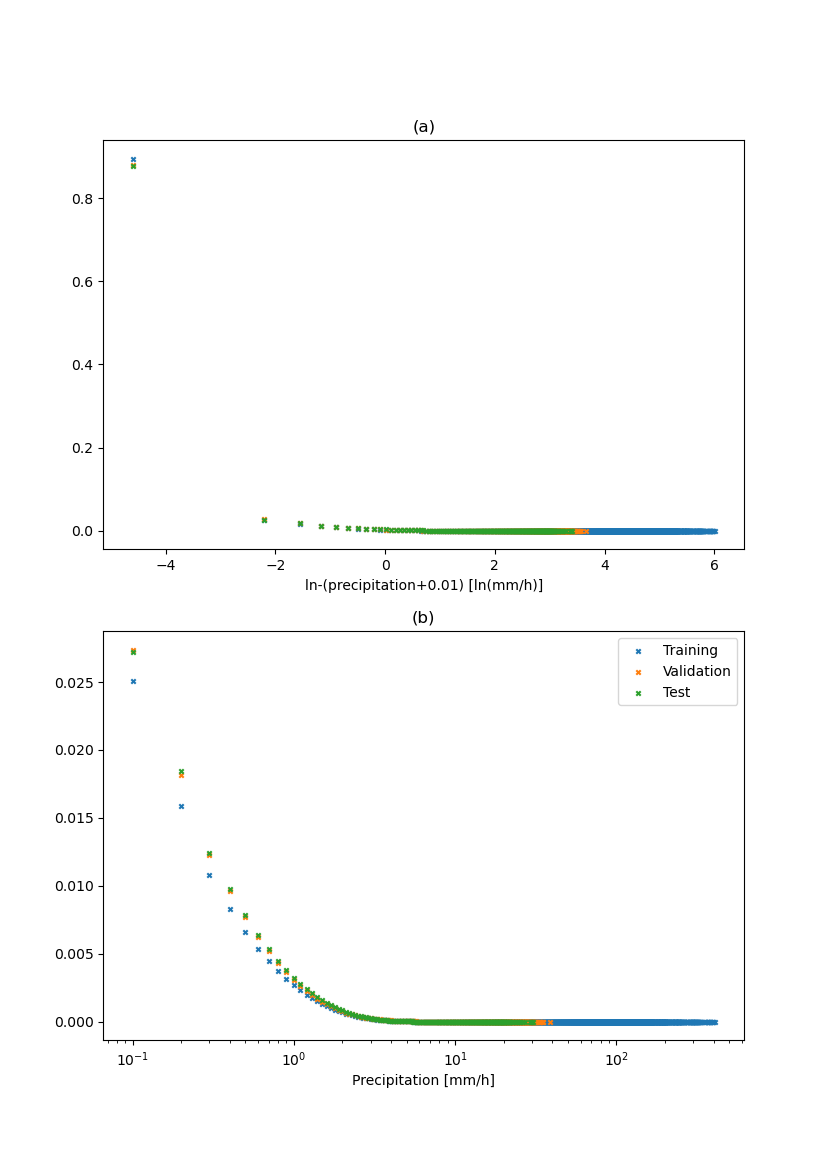
\includegraphics[width=0.9\textwidth]{figure_datasets.png}
    \caption{Relative frequency of all precipitation values for the pixels of the frames in the RADOLAN dataset. The distributions are computed for the training, validation ad test subsets of the dataset. (a) displays the distribution after the transformation of \cref{eq:transform}, hence the distribution of the values fed to the model. (b) is the distribution of the values displayed in log-scale without any addition but it does not contain the most frequent value 0 in order to better understand the distribution among the other values. }
    \label{fig:trainfreq}
\end{figure}


\section{Model Performance}
\subsubsection{Hyperparameter Search}\label{hyperparametersearch}
To avoid a computationally expensive procedure, the hyperparameters were divided in two groups. (1) Those manually tuned and (2) those picked by utilizing the available literature.

The manual search was done by trial and error considering all the metrics on the validation set, paying more attention to the HSS and the CSI. \cref{tab:hyperparameters} sums up the hyperparameters found through this process. 

\begin{table}[!h]
    \centering
    \begin{tabular}{cc}
        \hline
        \multicolumn{2}{c}{Hyperparameters} \\
        \hline
        \hline
         Name & Value \\
         batch size & 32 \\
         depth & 6 \\
         epochs & 10 \\
        \hline
    \end{tabular}
    \caption{The hyperparameters found via manual tuning.}
    \label{tab:hyperparameters}
\end{table}

\subsubsection{Testing}
Using the model produced through the hyperparameters of \cref{tab:hyperparameters} the metrics are computed on the testing subset. The results are summed up in \cref{tab:testing}

\begin{table}[!h]
    \centering
    \begin{tabular}{cccccc}
    \hline
    Metric & Cl. 0 & Cl. 0.1 & Cl. 1 & Cl. 2.5 & Macro average \\
     \hline
    \multirow{2}{*}{Precision} & \textbf{0.988} & 0.346 & \textbf{0.309} & 0.218 & 0.465 \\
         & 0.943 & \textbf{0.433} & 0.308 & \textbf{0.227} & \textbf{0.478}\\
    \hline
        \multirow{2}{*}{Recall} & 0.861 & \textbf{0.653} & \textbf{0.585} & \textbf{0.609} & \textbf{0.677} \\
         & \textbf{0.943} & 0.433 & 0.308 & 0.226 & 0.478 \\
    \hline
        \multirow{2}{*}{F1} & 0.921 & \bm{0.452} & \bm{0.404} & \bm{0.321} & \textbf{0.525} \\
         & \bm{0.943} & 0.432 & 0.308 & 0.227 & 0.478 \\
    \hline
        \multirow{2}{*}{CSI} & 0.853 & \bm{0.292} & \bm{0.253} & \bm{0.191} & \textbf{0.397} \\
         & \bm{0.893} & 0.276 & 0.182 & 0.128 & 0.370 \\
    \hline
        \multirow{2}{*}{HSS} & 0.579& 0.438 & \bm{0.404} & \bm{0.321} & \textbf{0.436} \\
         & \bm{0.583} & \bm{0.441} & 0.314 & 0.229 & 0.392 \\
    \hline
    \end{tabular}

    \caption{The results of the model compared to persistence applied to the test subset of the dataset. For every metric the upper row refers to the results of the model whilst the lower row refers to persistence. Higher values are better. The best values for each class and metric are highlighted.}
    \label{tab:testing}
\end{table}

As \cref{tab:testing} shows the performance of the model is generally better than persistence for higher precipitation classes suggesting an influence of the weights for the loss giving higher importance to higher precipitation. The generally high values for precision and recall for the lowest precipitation class can be explained by the overall higher amount of tiles with no precipitation making it an "easy guess". The most significant information is to be found in the overall better prediction skill of the model compared to persistence for the remaining classes as the macro-averages testify.

\begin{figure}[!h]
    \centering
    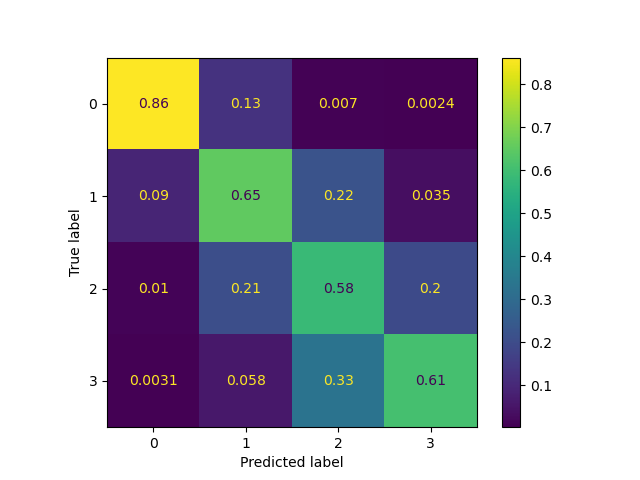
\includegraphics[width=0.9\textwidth]{normlized_confmatrix_test_2022-05-11 15:41:17.958023.png}
    \caption{The normalized confusion matrix for the predictions made by the model on the test set. Normalization occurs on the rows. The labels 0, 1, 2, 3 stand for the classes 0, 0.1, 1, 2.5 respectively.}
    \label{fig:confusion_matrix}
\end{figure}

\cref{fig:confusion_matrix} is the confusion matrix for the task. As it suggests the majority of wrong classifications happen with neighbouring classes, meaning that the model is able to understand the shape of the precipitation but has difficulties in assessing the intensity correctly.

\section{Case Studies}
To visually assess the goodness of the model I analyse two case studies, the first scene is the one at 2020-02-09T1950Z and the second one is at 2021-03-11T0150Z.

\subsection{First Case Study: 2020-02-09T1950Z}
\subsubsection{Synoptic Situation}
The synoptic situation near the time of the input and output of the neural network is addressed through the use of the model results produced by NOAA's model Global Forecast System (GFS)\footnote{https://www.ncei.noaa.gov/products/weather-climate-models/global-forecast} and visualized through Ertel2\footnote{http://ertel2.uibk.ac.at:8080/}. Geopotential height and equivalent potential temperature at 850hPa are employed. \cref{fig:ertel1} shows the relative figure for the model output at 2020-02-10T0000Z where the presence of a cold front is evident in the northern part of Germany near the area of interest (cf. \cref{fig:area_selection}). The orientation of the front is SW-NE. Additionally, given the orientation of the isolines representing the geopotential, the direction of the geostrophic flow is easterly. I also assess the 1h accumulated precipitation associated with this front by observing the output of the ICON (EU) model\footnote{more on the ICON (EU) model to be found at \newline \hyperlink{https://www.dwd.de/EN/ourservices/nwp\_forecast\_data/nwp\_forecast\_data.html}{https://www.dwd.de/EN/ourservices/nwp\_forecast\_data/nwp\_forecast\_data.html}} through Ventusky\footnote{\hyperlink{https://www.ventusky.com/}{https://www.ventusky.com/}} at 2020-02-10T0300Z. \cref{fig:ventusky1} shows the relative image. The precipitation bands near the area of interest in northern Germany (again cf. \cref{fig:area_selection}) are oriented in a similar direction to the cold front i.e. SW-NE.
\begin{figure}[!h]
    \centering
    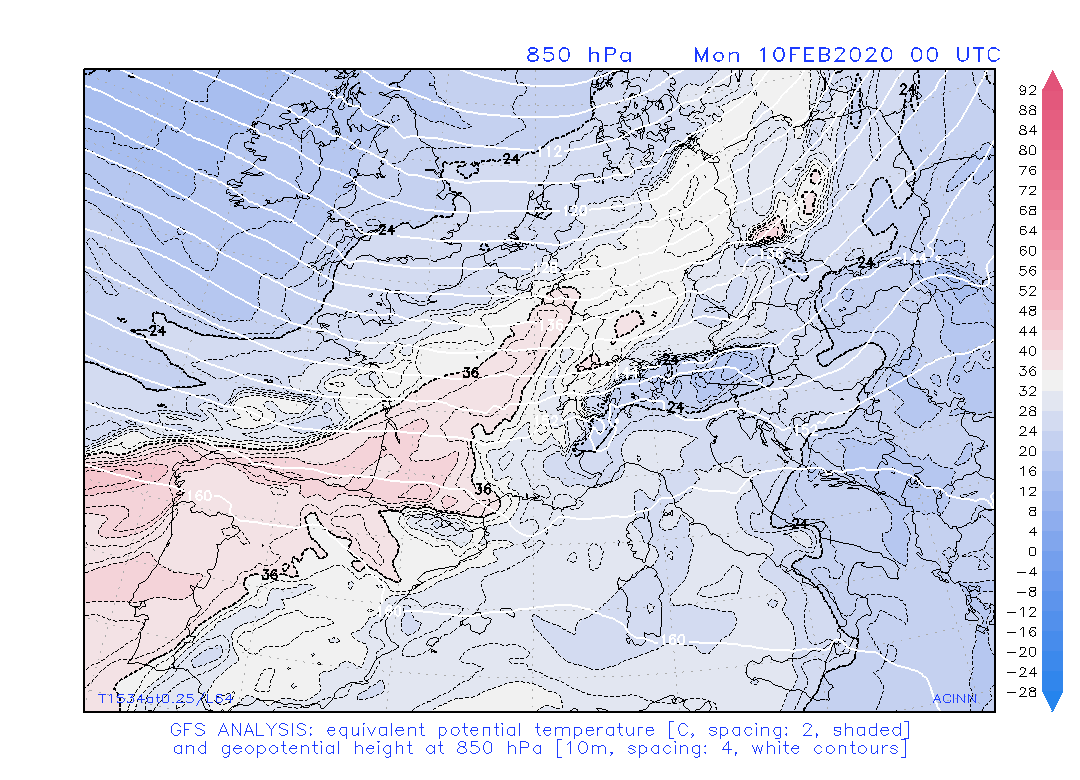
\includegraphics[width=0.9\textwidth]{2002100000_gfs.png}
    \caption{Output of the GFS model for the timestamp 2020-02-10T0000Z showing equivalent potential temperature and geopotential height at 850hPa. The equivalent potential temperature is in C, shaded and with lines at 2\textdegree C distance. The geopotential height is shown in white contours and in 10m units. The spacing between the lines is 4. The SW-NE cold front in the area of interest in norther Germany is evident. The flow is assessed through the geopotential height and is easterly. Figure produced with the help of ERTEL2.}
    \label{fig:ertel1}
\end{figure}
\begin{figure}
    \centering
    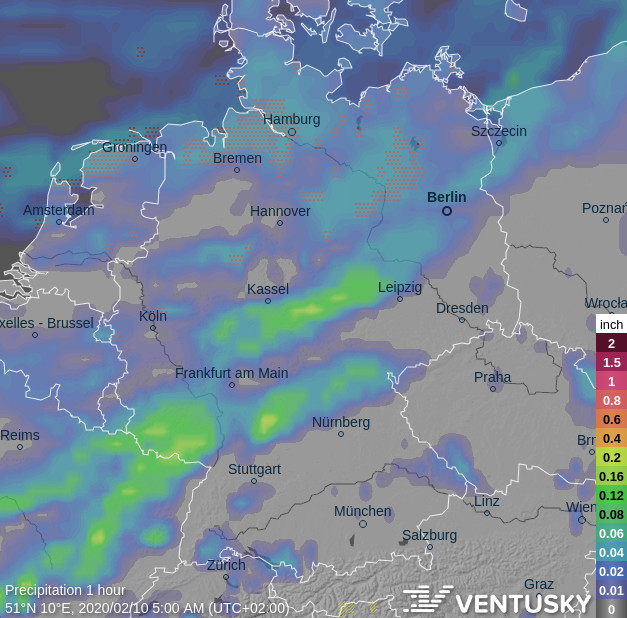
\includegraphics[width=0.9\textwidth]{ventusky-rain-1h-20200210t0300-51n10e.jpg}
    \caption{1h precipitation over Germany at 2020-02-10T0300Z according to the ICON (EU) model. The frontal structure after it has passed over the area of interest and its approximate SW-NE orientation can be seen clearly. Figure produced with Ventusky.}
    \label{fig:ventusky1}
\end{figure}

\subsubsection{Model Prediction}
Following the synoptic situation described in the previous section I analyze the actual output of the model given the input sequence. \cref{fig:examplescene1} shows the scene for 2020-02-09T1950Z. This timestamp is the timestamp of the first input image (upper left in the group of 6 images). The other 5 input images are those depicted in the group made of 6 images in \cref{fig:examplescene1} and all are of precipitation accumulated in a 1h interval. They are separated by 1h from each other. The model then applies a series of convolutions (cf \cref{sec:convolutional_layers}) that abstract the features of the input images in a representational space that the model itself learns during the training process. The spatial resolution is reduced for every layer that the input data goes through in the encoding phase (cf. \cref{sec:Unet}) but is later taken back to the original resolution in the decoding phase. In this last phase the model rebuilds a plausible output image using information from the encoding phase thanks to the skip connections (cf. \cref{sec:skip_connections}). The timestamp of the output of the model is 6h after the first input image, hence 2020-02-10T0150Z and it is shown in the last row on the left of \cref{fig:examplescene1}, it is confronted with the ground truth on the same row on the right. This allows for a straightforward comparison and shows if the model has acquired the ability to infer the spatial distribution of the precipitation correctly. As \cref{fig:examplescene1} shows the model is indeed able to predict precipitation rainbands going in the SW-NE direction as is seen in the ground truth and in \cref{fig:ventusky1}. However, it is clear that the model predicts higher precipitation rates than are actually observed. An hypothesis for this behaviour is the influence of the weights employed for the loss that give very high importance to higher precipitation rates.
\begin{figure}[!h]
    \centering
    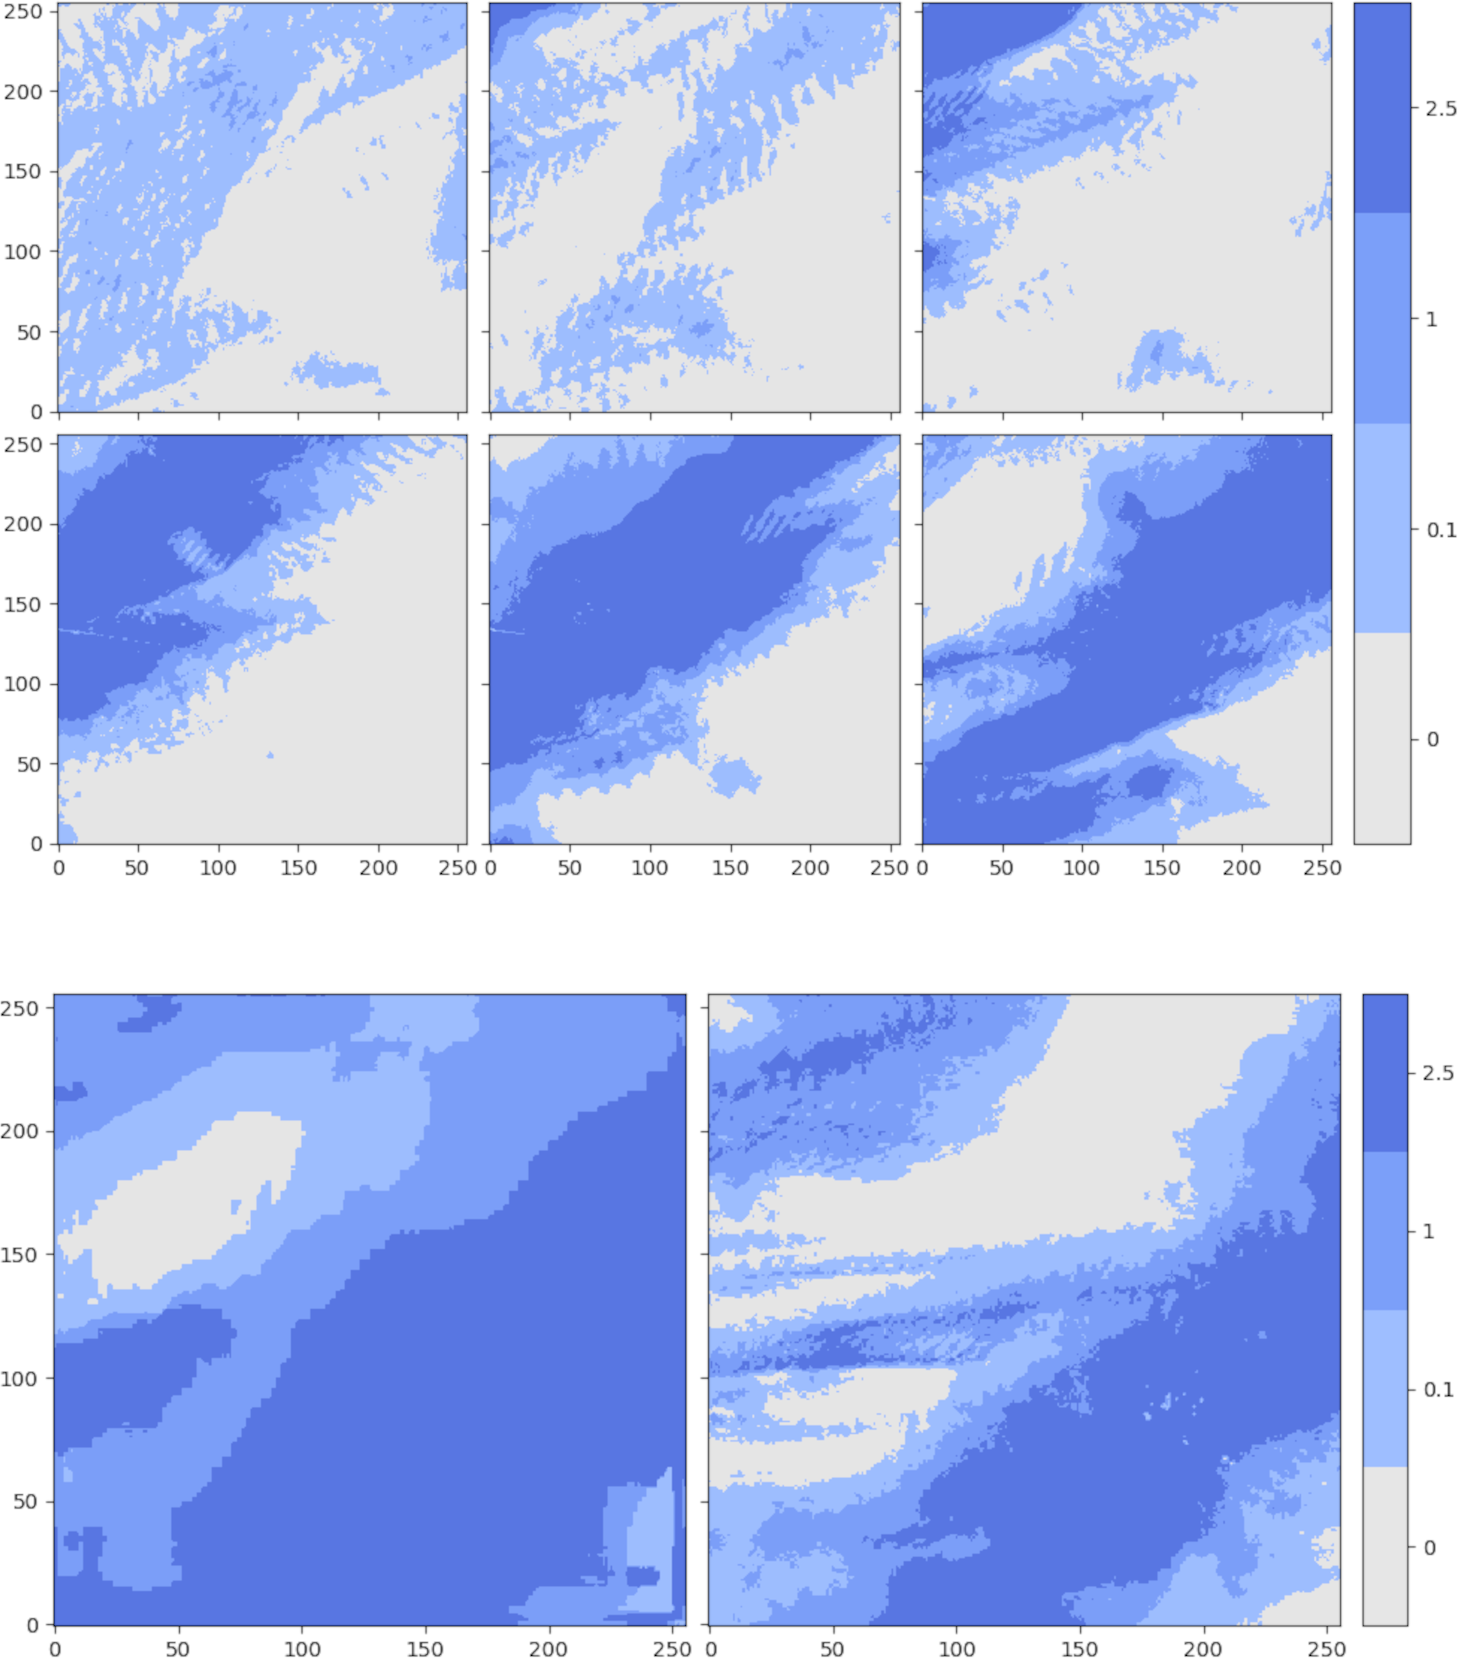
\includegraphics[width=0.9\textwidth]{2002091950.png}
    \caption{Example of input and output and ground truth for 2020-02-09T1950Z. The input part is made of the six images in the top. The prediction is the left image of the lower two and the ground truth is to be found on the right of the prediction. The input is fed to the model as continuous precipitation values but it is depicted in precipitation classes to better compare them with the output. The labels on the right refer to the precipitation classes. The coordinates are in km from the bottom left corner. The order of the inputs is left to right top to bottom. The interval between every one is one hour and all are 1h cumulative precipitation values. The model can be seen to correctly predict the orientation of the precipitation bands. At the same time it predicts higher precipitation values than the ground truth.}
    \label{fig:examplescene1}
\end{figure}

\subsection{Second Case Study: 2021-03-11T0150Z}
\subsubsection{Synoptic Situation}
Similarly to the first case study, I assess the synoptic situation at a time approximately near to the input and output of the neural network (the latter is 6h after the input image, hence 2021-03-11T0750Z) using the same tools. \cref{fig:ertel2} shows the output of GFS and shows the presence of a warm front that is starting to enter the area of interest in northern Germany at 2021-03-11T0000Z. Its orientation is S-N. The geostrophic flow associated to the system, being parallel to the isolines of geopotential height, is found to be easterly to south-easterly. The rainbands associated with this front can be seen in the ICON (EU) model output taken at 2021-03-11T0900Z after they have left the area of interest and are in the SW-NE direction.
\begin{figure}[!h]
    \centering
    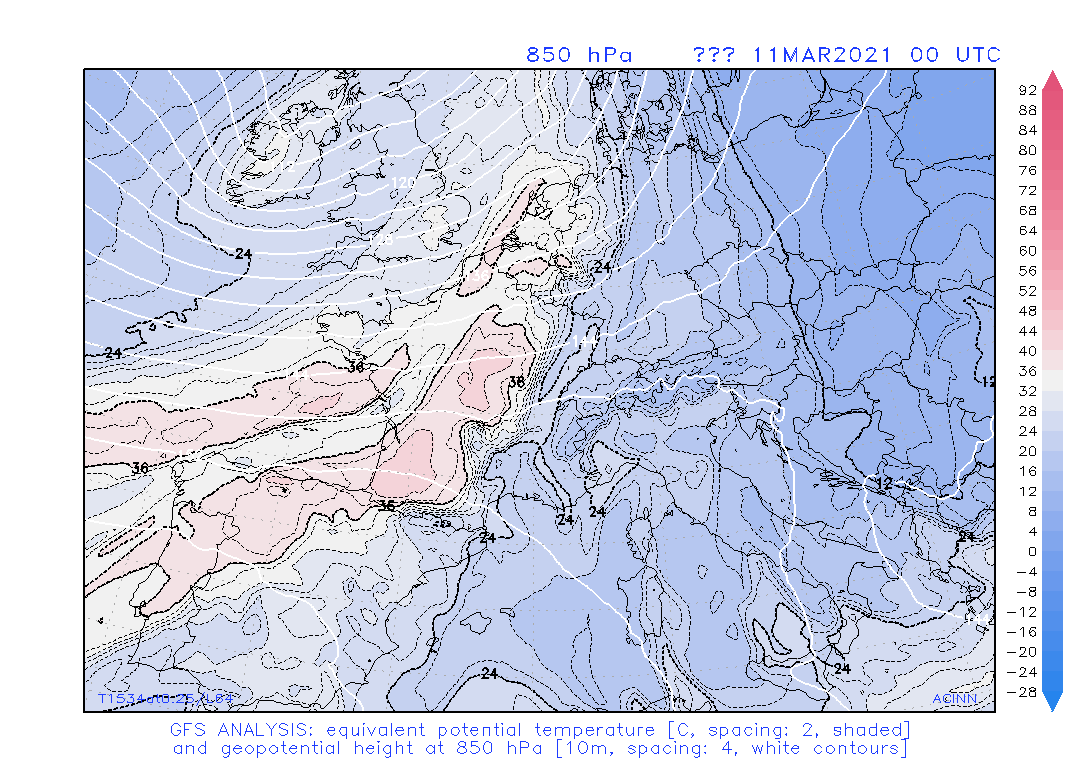
\includegraphics[width=0.9\textwidth]{2103110000_gfs.png}
    \caption{Output of the GFS model for the timestamp 2020-03-11T0000Z showing equivalent potential temperature and geopotential height at 850hPa. The equivalent potential temperature is in C, shaded and with lines at 2\textdegree C distance. The geopotential height is shown in white contours and in 10m units. The spacing between the lines is 4. The N-S warm front approaching the area of interest in northern Germany is evident. The geostrophic flow, parallel to the isolines of geopotential height, is easterly to south-easterly. Figure produced with the help of ERTEL2.}
    \label{fig:ertel2}
\end{figure}
\begin{figure}
    \centering
    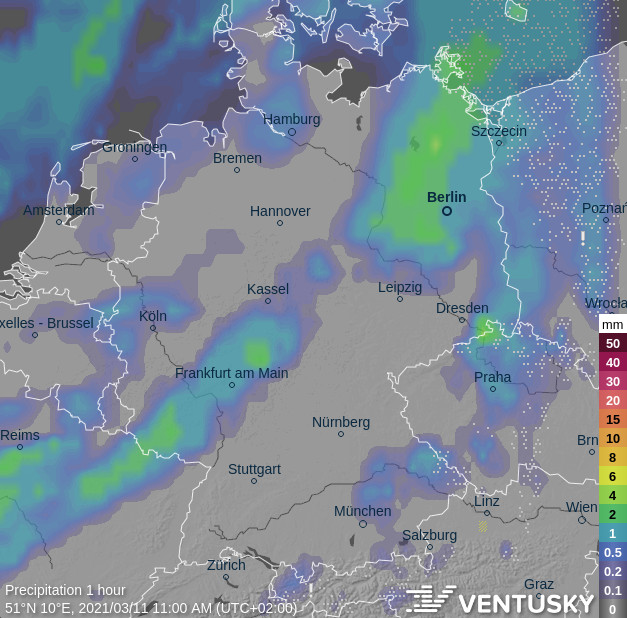
\includegraphics[width=0.9\textwidth]{ventusky-rain-1h-20210311t0900-51n10e.jpg}
    \caption{1h precipitation over Germany at 2021-03-11T0900Z according to the ICON (EU) model. The frontal structure after it has passed over the area of interest can be seen over northern Germany. Its orientation is SW-NE. Figure produced with Ventusky.}
    \label{fig:ventusky2}
\end{figure}

\subsubsection{Model Prediction}
Following the synoptic situation, I assess again the ability of the model to predict high level features such as the direction of the precipitation bands. I find in \cref{fig:examplescene2}, similarly to the first case, that the model is able to predict the direction of the precipitation bands but outputs higher precipitation rates than the ground truth.
\begin{figure}[!h]
    \centering
    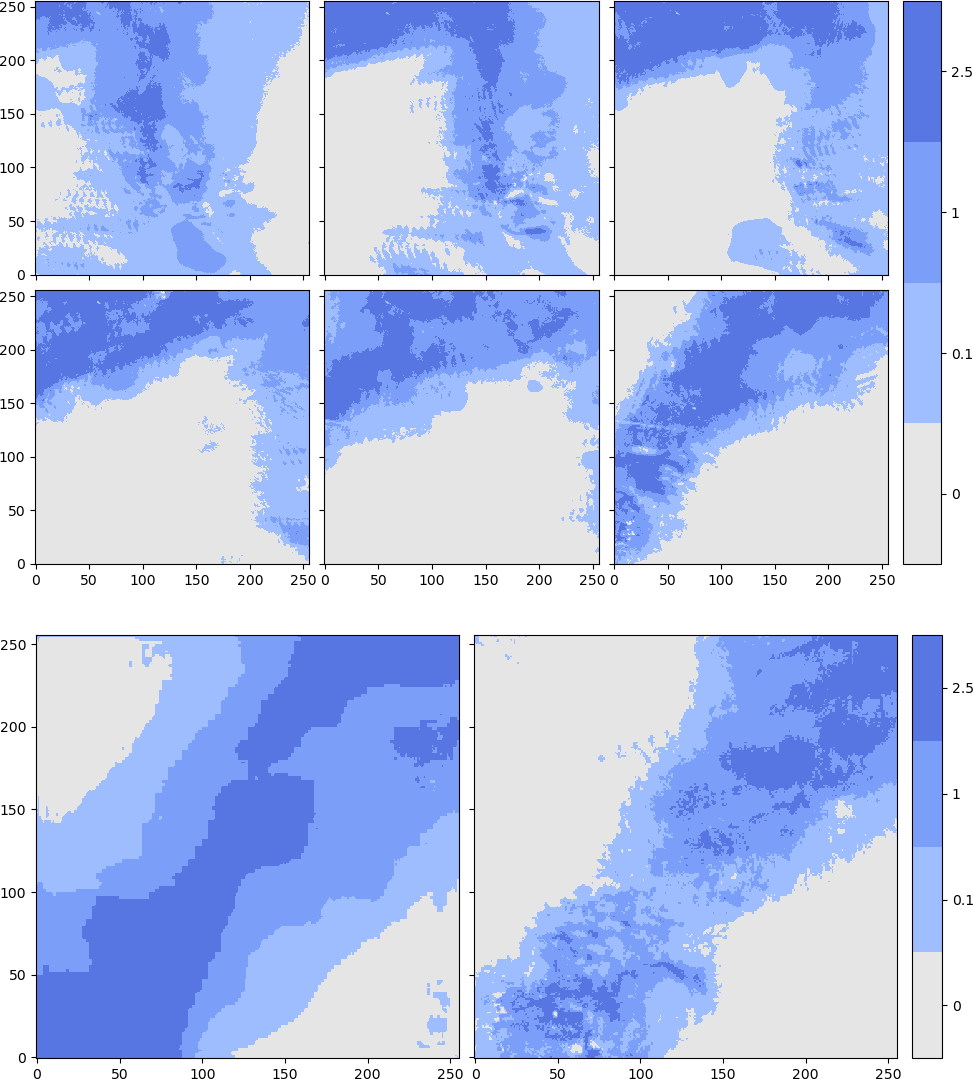
\includegraphics[width=0.9\textwidth]{2103110150.png}
    \caption{Example of input and output and ground truth for 2021-03-11T0150Z. The input part is made of the six images in the top. The prediction is the left image of the lower two and the ground truth is to be found on the right of the prediction. The input is fed to the model as continuous precipitation values but it is depicted in precipitation classes to better compare them with the output. The labels on the right refer to the precipitation classes. The coordinates are in km from the bottom left corner. The order of the inputs is left to right top to bottom. The interval between every one is one hour and all are 1h cumulative precipitation values. The model can be seen to correctly predict the orientation of the precipitation bands. At the same time it predicts higher precipitation values than the ground truth.}
    \label{fig:examplescene2}
\end{figure}

